\documentclass[tikz,border=5mm]{standalone}
\begin{document}
	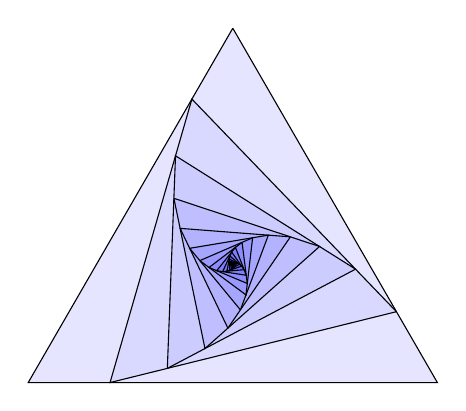
\begin{tikzpicture}
		\def\n{3}
		\def\r{3}
		\def\pos{.2}
		\colorlet{mycolor}{blue}
		\foreach \i in {1,...,\n}
		\path ({90+360*\i/\n}:\r) coordinate (A\i);
		\path (A\n) coordinate (T);
		\draw[fill=mycolor!10] (T) foreach \i in {1,...,\n} {--(A\i)};
		\foreach \k in {1,2,...,50}{
			\pgfmathsetmacro{\kcolor}{10+5*\k}
			\path (T) foreach \i in {1,...,\n}
			{--(A\i) coordinate[pos=\pos] (A\i)};
			\path (A\n) coordinate (T);
			\draw[fill=mycolor!\kcolor] (T) foreach \i in {1,...,\n} {--(A\i)};
		}
	\end{tikzpicture}
\end{document}
